\section{Introduction}
\label{network:kerberos:authentication}

\subsection{major Components}

The Kerberos protocol defines how  clients interact with a network authentication service. Clients obtain  tickets from the Kerberos Key Distribution Center (KDC), and they submit  these tickets to application servers when connections are established.  It uses UDP port 88 by default and depends on the process of symmetric  key cryptography.
“Kerberos uses tickets to authenticate a user and completely avoids sending passwords across the network”.
There are some key components in Kerberos authentication that play a crucial role in the entire authentication process.
\begin{figure}[!ht]
  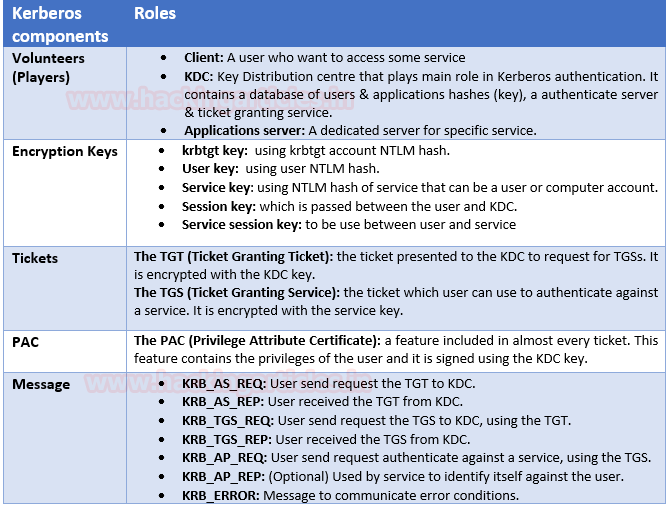
\includegraphics[width=\linewidth]{network/kerberos/images/kerb-components.png}
  \caption{Kerberos components}
  \label{fig:kerberos-components}
\end{figure}

\subsection{Workflow}

In the Active Directory domain, every  domain controller runs a KDC (Kerberos Distribution Center) service that  processes all requests for tickets to Kerberos. For Kerberos tickets,  AD uses the KRBTGT account in the AD domain.
The image below shows that the major  role played by KDC in establishing a
secure connection between the  server \& client and the entire process uses some special components  as defined in the table above.

\begin{figure}[!ht]
  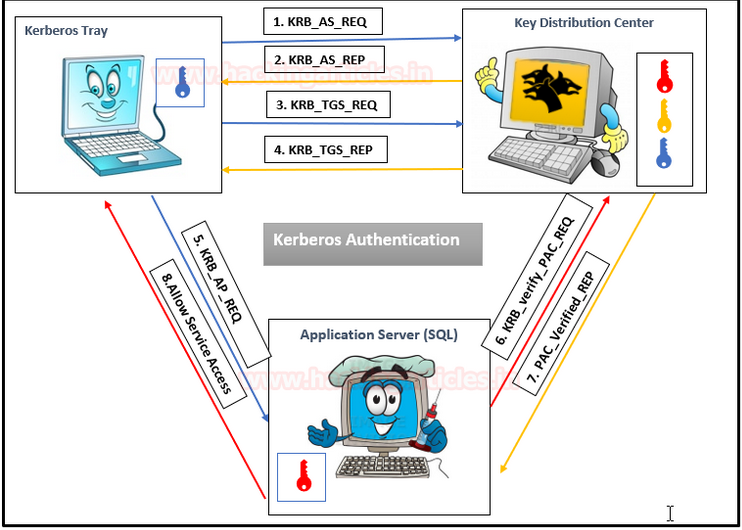
\includegraphics[width=\linewidth]{network/kerberos/images/kerb-all.png}
  \caption{Kerberos Workflow}
  \label{fig:kerberos-workflow}
\end{figure}


As mentioned above, Kerberos uses  symmetric cryptography for encryption and decryption. Let us get into  more details and try to understand how encrypted messages are sent to  each other. Here we use three colours to distinguish Hashes:
\begin{itemize}
    \item \verb+BLUE _KEY+: User NTLM HASH
    \item \verb+YELLOW_KEY+: Krbtgt NTLM HASH
    \item \verb+RED_KEY+: Service NTLM HASH
\end{itemize}

\subsubsection*{Step 1: Communication initialization}
\verb+KRB_AS_REQ+ contains the following:
\begin{itemize}
    \item Username of the client to be authenticated.
    \item The service SPN (SERVICE PRINCIPAL NAME) linked with Krbtgt account
    \item An encrypted timestamp (Locked with User Hash: Blue Key)
\end{itemize}

The entire message is encrypted using the User NTLM hash (Locked with BLUE KEY) to authenticate the user and prevent replay attacks.

\subsubsection*{Step 2}

The KDC uses a database consisting of Users/Krbtgt/Services hashes to decrypt a message (Unlock with BLUE KEY) that authenticates user identification.
Then KDC will generate TGT (Ticket  Granting Ticket) for a client that is
encrypted using Krbtgt hash  (Locked with Yellow Key) \& some Encrypted Message using User Hash.

\verb+KRB_AS_REP+ contains the following:
\begin{itemize}
    \item  Username
    \item  Some encrypted data, (Locked with User Hash: Blue Key) that contains: 
    \begin{itemize}
        \item  Session key
        \item  The expiration date of TGT
    \end{itemize}
    \item  TGT, (Locked with Krbtgt Hash: Yellow Key) which contains:
    \begin{itemize}
        \item  Username
        \item  Session key
        \item  The expiration date of TGT
        \item  \gls{win:PAC}~\ref{network:ad:kerberos:PAC}
 with user privileges, signed by KDC
    \end{itemize}
\end{itemize}

\begin{figure}[!ht]
  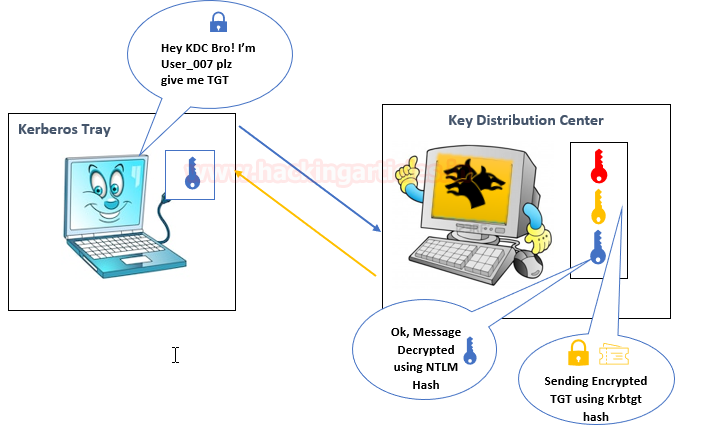
\includegraphics[width=\linewidth]{network/kerberos/images/kerb-1.png}
  \caption{Kerberos TGT}
  \label{fig:kerberos-tgt}
\end{figure}

\begin{figure}[!ht]
  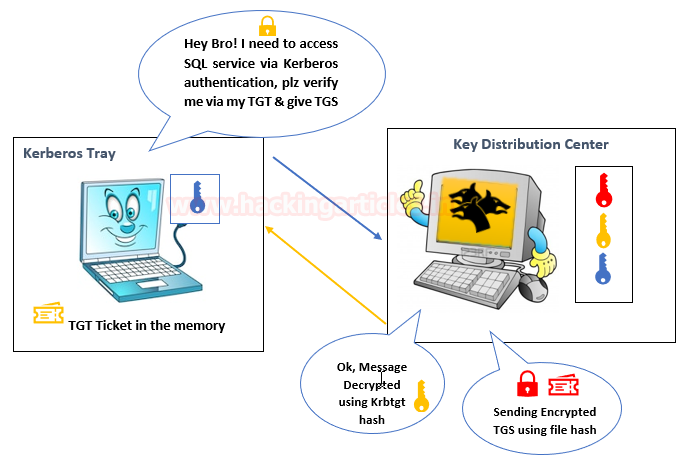
\includegraphics[width=\linewidth]{network/kerberos/images/kerb-2.png}
  \caption{Kerberos TGS}
  \label{fig:kerberos-tgs}
\end{figure}

\begin{figure}[!ht]
  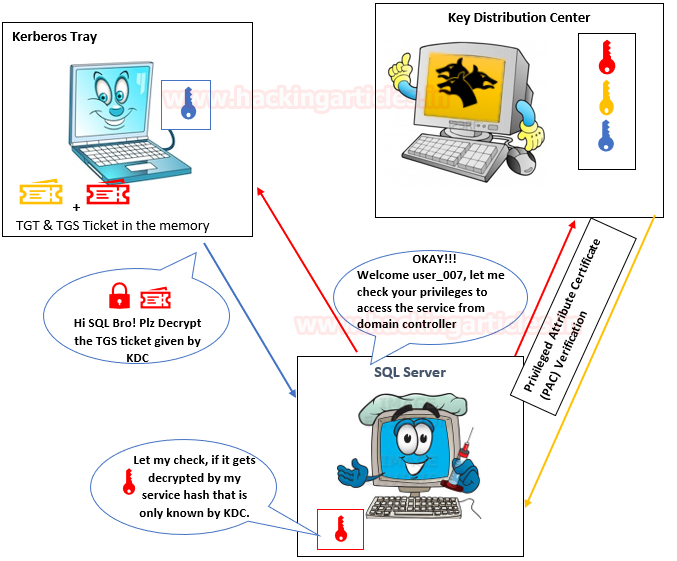
\includegraphics[width=\linewidth]{network/kerberos/images/kerb-3.png}
  \caption{Kerberos Service Authentication}
  \label{fig:kerberos-service}
\end{figure}

\subsubsection*{Step 3}
The \verb+KRB_TGT+ will be stored in the Kerberos tray (Memory) of the client
machine, as the user already has the \verb+KRB_TGT+, which is used to identify  himself for the TGS request. The client sent a copy of the TGT with the  encrypted data to KDC.

\verb+KRB_TGS_REQ+ contains:
\begin{itemize}
    \item Encrypted data with the session key
    \begin{itemize}
        \item Username
        \item Timestamp
    \end{itemize}
    \item TGT
    \item SPN of requested service e.g. SQL service
\end{itemize}


\subsubsection*{Step 4}

The KDC receives the \verb+KRB_TGS_REQ+ message and decrypts the message using
Krbtgt hash to verify TGT (Unlock using Yellow key), then KDC returns a  TGS as
\verb+KRB_TGS_REP+ which is encrypted using requested service hash (Locked with
Red Key) and Some Encrypted Message using User Hash.

\verb+KRB_TGS_REP+ contains:
\begin{itemize}
    \item Username
    \item Encrypted data with the session key:
    \begin{itemize}
        \item Service session key
    \end{itemize}
    \item The expiration date of TGS
    \item TGS, (Service Hash: RED Key) which contains:
    \begin{itemize}
        \item  Service session key
        \item Username
        \item The expiration date of TGS
        \item  \gls{win:PAC}~\ref{network:ad:kerberos:PAC}
 with user privileges, signed by KDC
    \end{itemize}
\end{itemize}


\subsubsection*{Step 5}
The user sent the copy of TGS to the Application Server,\verb+KRB_AP_REQ+ contains:
\begin{itemize}
    \item TGS
    \item Encrypted data with the service session key:
    \begin{itemize}
        \item Username
        \item Timestamp, to avoid replay attacks
    \end{itemize}
\end{itemize}

\subsubsection*{Step 6}
The  application attempts to decrypt the message using its NTLM hash and to  verify the PAC from KDC to identify user Privilege which is an optional  case.
\subsubsection*{Step 7}
KDC verifies PAC (Optional)
\subsubsection*{Step 8}
Allow the user to access the service for a specific time.

\subsection{Kerberos authentication to a parent domain}
When a two-way trust is created, a user account is created in each domain where the username is set to the NetBIOS domain name of the other domain followed by \verb+$+. The same password is set on both accounts, resulting in identical Windows NT hashes and Kerberos RC4 secret keys for the two accounts. The Kerberos AES secret keys are not identical as these keys are generated with a cryptographic salt containing the domain and username, which are different for the two accounts. 

mimikatz: \verb+lsadump::lsa /inject /user:<domain>$+

The trust account’s passwords are used as shared secrets between the domains, and the {\bf trust account’s Kerberos secret keys derived from the passwords are used as inter-realm trust keys}, which are the keys {\bf used for encryption of Kerberos tickets between the domains}. The AES secret keys of the trust accounts are not identical to the AES inter-realm trust keys, as a different cryptographic salt is used.

mimikatz: \verb+lsadump::trust /patch+



A DC holds only the Kerberos secret keys of the AD accounts of the domain the DC belongs to. So, when a user asks for access to a service outside of the domain, the KDC cannot access the secret key of the service account in the other domain and thereby can’t create an encrypted service ticket. 

\begin{figure}[!ht]
  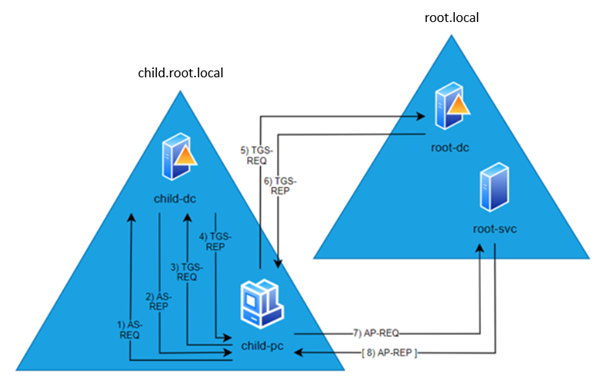
\includegraphics[width=\linewidth]{network/kerberos/images/Picture17.png}
  \caption{inter-realm protocol}
  \label{fig:kerberos-inter-realm}
\end{figure}

The steps are the same as Kerberos authentication inside a single domain, except TGS Exchange with the parent KDCc has been added. Yet another TGS Exchange would be added if the authentication was to a service of a third domain with a trust relationship with the parent domain e.g. a sibling domain to the child.

\subsubsection{AS Exchange}

{\bf TGT PAC} contains:
\begin{itemize}
    \item LogonDomainId: SID of client user domain
    \item UserId: RID of client user
    \item PrimaryGroupId: RID of client user’s primary group
    \item UserFlags:  bit flags describing the user logon and other stuff. The flag \verb+D+ is set: “Indicates that the ExtraSids field is populated and contains additional SIDs”.
    \item GroupIds: The list contains the RIDs of global and universal groups of the client user domain of which the client user is a member. The list contains only the RIDs and not the SIDs, as all the groups begin with domain SID which is in the LogonDomainId attribute. This makes the PAC smaller in bytes. Note that domain local groups are not in this list. More on that when we get to the service ticket.
    \item {\bf ExtraSids}: contains SIDs of groups/identities of the client user which does not begin with the domain SID. That is:
        \begin{itemize}
            \item 
                SIDs of universal groups of other domains
            \item
                SID history SIDs
            \item
                Other identities (e.g. S-1-18-1 Authentication authority asserted identity)
            \item
                The SID S-1-18-1 is mandatory. It means the client's identity is asserted by an authentication authority based on proof of possession of client credentials. It was introduced in Windows 8 / Server 2012.
        \end{itemize}
    \item
        {\bf SidCount}: Number of SIDs in ExtraSids
    \item ResourceGroupDomainSid: NULL
    \item ResourceGroupIds: NULL
    \item ResourceGroupCount: 0
\end{itemize}

\subsubsection{TGS Exchange (child KDC)}
{\bf TGS-REQ} :
Since the domain name of the service is different from the child domain name, the client user will include the option \verb+NAME_CANONICALIZE+ in the \verb+TGS-REQ+ to indicate the service may be in another domain.

{\bf TGS-REP} :
sends back a TGS-REP of the type {\bf TGS referral} containing:
\begin{itemize}
    \item Pre-authentication data: The Pre-authentication type \verb+PA-SVR-REFERRAL-INFO+ indicates the message is a referral. Where the normal \verb+PA-ENC-TIMESTAMP+ pre-authentication contains the client user’s name and a timestamp, \verb+PA-SVR-REFERRAL-INFO+ contains the client user’s name and the name of the parent domain.
    \item An {\bf inter-realm TGT}: A TGT encrypted with an inter-realm trust key derived from the \verb+ROOT$+ trust account password (instead of krbtgt’s secret key). By default, the RC4 trust key is used. As a regular TGT, this TGT contains a TGS session key, but for the TGS Exchange with the parent domain. The PAC of this TGT is a copy of the PAC from the TGT sent by the client user in the TGS-REQ.
    \item Ticket information: he information indicates that the response is a referral to the TGS of the parent domain. The ticket information is encrypted with the TGS session key retrieved by the TGS from the TGT sent by the client user in the TGS-REQ.
    \item A TGS session key: The session key for the TGS Exchange with the parent domain. It is encrypted with the TGS session key retrieved by the TGS from the TGT sent by the client user in the TGS-REQ
\end{itemize}

The PAC of the inter-realm ticket is a complete copy of the TGT PAC, as stated in the MS-KILE TGS Exchange documentation: “The KILE KDC MUST copy the populated fields from the PAC in the TGT to the newly created PAC …”. The TGS Exchange specifies also that the PAC must be populated with domain local group membership for the client user, except for inter-realm TGTs. No validation of the TGT PAC data seems to be performed.


\subsubsection{TGS Exchange (parent KDC)}

{\bf TGS-REQ}:
The client user decrypts the ticket information and realizes that the TGS-REP is a referral. The client user sends a new TGS-REQ, this time to the parent domain, with the \verb+NAME_CANONICALIZE+ option again. The TGS-REQ contains:
\begin{itemize}
    \item An authenticator: The authenticator contains the pre-authentication data send by the child domain TGS in the TGS-REP. The client user has encrypted the authenticator using the TGS session key also received from the child domain TGS TGS-REP.
    \item The inter-realm TGT
\end{itemize}

{\bf TGS-REP}:
The KDC of the parent domain realizes that the TGS-REQ is a referral by the \verb+PA-SVR-REFERRAL-INFO+ pre-authentication type and decrypts the inter-realm TGT using its copy of the inter-realm trust key. The parent domain TGS gets access to the TGS sessions key from the inter-realm TGT and decrypts and verifies the authenticator. If the authenticator is valid, the TGS replies to the user client with a TGS-REQ containing:
\begin{itemize}
    \item An AP session key: The AP session key is encrypted with the TGS session key.
    \item A service ticket: The service ticket contains a copy of the AP session key and a copy of the user’s PAC from the inter-realm TGT. The PAC has been extended with authorization data from this domain i.e. domain local group memberships of this domain. The service ticket is encrypted using the secret key of the service account.
\end{itemize}

When the parent KDC creates a service ticket the PAC is again copied, but this time the PAC is populated with domain local groups. This updates some of the PAC attributes:
\begin{itemize}
    \item UserFlags: In addition to flag \verb+D+, UserFlags now has flag \verb+H+ set which “Indicates that the ResourceGroupIds field is populated.”
    \item ResourceGroupDomainSid: SID of parent domain
    \item ResourceGroupIds: The list contains the RIDs of domain local groups of the parent domain of which the client user is a member. Global groups of the parent domain are neither in this attribute nor ExtraSids as global groups cannot contain members of other domains
    \item ResourceGroupCount: Number of RIDs in ResourceGroupIds
\end{itemize}



From the MS documentation, it seems like entries present in ResourceGroupIds of the inter-realm TGT PAC are copied to the service ticket PAC, but our tests with forged tickets showed that our entries in ResourceGroupIds of the inter-realm TGT were removed from the PAC by the parent domain TGS and not present in the service ticket. However, all SIDs in the ExtraSids remain.


\subsubsection{AP Exchange}
The client user uses the TGS-REP data to initiate an AP Exchange like the AP Exchange of a normal intra-domain Kerberos authentication, where the service account gives access based on the PAC of the service ticket.

The service account creates an \verb+ImpersonationAccessToken+ and populates it with the SIDs of the PAC attributes in the service ticket, and determines which access the client user has. Optional PAC validation gives the option to send a checksum of the PAC from the service account to the parent KDC to make sure it is not a forged service ticket but is not performed by default. This validation is also limited, as it will not catch if the TGT or the inter-realm TGT was forged, only forged service tickets.

\subsection{Privileged Attribute Certificate (PAC)}
\label{network:ad:kerberos:PAC}

The \gls{win:PAC} is an extension to Kerberos tickets that contains useful
information about a user’s privileges.  This information is added to Kerberos
tickets by a domain controller when a user authenticates within an Active
Directory domain.  When users use their Kerberos tickets to authenticate to
other systems, the PAC can be read and used to determine their level of
privileges without reaching out to the domain controller to query for that
information (more on that to follow).

PACs contain very sensitive information and therefore have been the target of
several Active Directory attack techniques over the years.

PAC is double encrypted (SPN hash) signed by the KDC hash.

Critical services in term of perf (MSSQL) don't ask the KDC to verify this open
to PAC forgery attack

\url{https://stealthbits.com/blog/what-is-the-kerberos-pac/}


\subsection{Service Principal Name (SPN)}
\label{network:ad:kerberos:SPN}
\index{Active Directory!SPN}

\gls{win:SPN}s are unique identifiers that Kerberos uses to map a service
instance to a service account in whose context the service is running. Domain
accounts are often used to run services to overcome the network authentication
limitations of built-in accounts such as \verb+NT AUTHORITY\LOCAL SERVICE+

Active Directory Domain  Services and Windows provide support for Service Principal Names (SPNs),  which are key components of the Kerberos mechanism through which a  client authenticates a service.

Domain accounts running services are often local administrators, if not highly
privileged domain accounts. Due to the distributed nature of systems,
interacting services, and associated data transfers, service accounts may be
granted administrator privileges on multiple servers across the enterprise.
Many services require elevated privileges on various systems, so service
accounts are often added to privileged groups, such as Domain Admins, either
directly or via nested membership. {\bf Finding SPNs associated with highly
privileged accounts in a Windows environment is very common}. 

Important Points:
\begin{enumerate}
\item If you install multiple instances of a service on computers throughout a forest, each instance must have its SPN. 
\item Before the Kerberos authentication service can use an SPN to authenticate a service, the SPN must be registered on the account.
\item A given SPN can be registered on only one account. 
\item An SPN must be unique in the forest in which it is registered.
\item If it is not unique, authentication will fail.
\end{enumerate}

\subsubsection{SPN format}
\verb+<ServiceClass>/<host>:<port>/<arbitratyName>+
\begin{itemize}
    \item \verb+ServiceClass+: \verb+HTTP, LDAP,MSSQLSVC+ \ldots 
    \item \verb+host+:\verb+fqdn+ or \verb+hostname+ or \verb+<DomainName>/<MachineName>+ 
\end{itemize}

\href{https://beta.hackndo.com/service-principal-name-spn/}{hackndo SPN explained}

\subsubsection{Type of SPN}
\begin{itemize}
\item Host-based SPNs which is associated  with the computer account in AD, it is randomly generated 128-character  long password which is changed every 30 days, hence it is no use in  Kerberoasting attacks
\item SPNs that have been associated with a domain user account where NTLM hash will be used.
\end{itemize}

\subsection{Pre-authentication}
\label{windows:authentication:kerberos:preauthentication}

Pre-authentication requires that requestors prove their identity before the KDC will issue a ticket for a particular principal. There are several types of pre-authentication defined by the Kerberos Clarifications document. However, only the  encrypted timestamp (PA-ENC-TIMESTAMP) pre-authentication method is commonly implemented.

Pre-authentication is controlled by KDC policy. If a user attempts to acquire
initial tickets through the AS exchange, but the KDC requires
pre-authentication, then the KDC will send a \verb+KRB_ERROR+ message instead
of an \verb+AS_REP+ in reply to the client AS request. This \verb+KRB_ERROR+ message tells the client that pre-authentication is required. If the KDC responds with the error \verb+PRINCIPAL UNKNOWN+, the username is invalid.

This request used for username enumeration does not cause logon failures and will not
lock out accounts.



After the enumeration of user accounts is finished, we can attempt to abuse a
feature within Kerberos with an attack method called \verb+ASREPRoasting+. ASReproasting occurs when a user account has the privilege "Does not require Pre-Authentication" set. This means that the account does not need to provide valid identification before requesting a Kerberos Ticket on the specified user account.

The Kerberos protocol defines how  clients interact with a network authentication service. Clients obtain  tickets from the Kerberos Key Distribution Center (KDC), and they submit  these tickets to application servers when connections are established.  It uses UDP port 88 by default and depends on the process of symmetric  key cryptography.
“Kerberos uses tickets to authenticate a user and completely avoids sending passwords across the network”.
There are some key components in Kerberos authentication that play a crucial role in the entire authentication process.

This method does not generate Windows event ID
\href{https://docs.microsoft.com/en-us/windows/security/threat-protection/auditing/event-4625}{4625:
An account failed to log on}, or a logon failure which is often monitored for.

\url{https://ldapwiki.com/wiki/Kerberos%20Pre-Authentication}

\subsection{Kerberos on Linux}
\url{https://www.techblog.moebius.space/posts/2018-05-25-kerberos-an-overview-of-principals-and-keytabs/#keytabs}


In most cases, Linux machines store Kerberos tickets as \verb+ccache+ files in
the \verb+/tmp+ directory. By default, the location of the Kerberos ticket is
stored in the environment variable \verb+KRB5CCNAME+.
These
\href{https://web.mit.edu/kerberos/krb5-1.12/doc/basic/ccache_def.html}{ccache}
files are protected by reading and write permissions, but a user with elevated
privileges or root privileges could easily gain access to these tickets.

Another everyday use of Kerberos in Linux is with
\href{https://kb.iu.edu/d/aumh}{keytab} files.

\subsubsection{Keytabs}
In most cases, end-users would authenticate to the KDC using their  client
secret (i.e their password). However, it would be cumbersome for  automated
scripts and applications to regularly (re)authenticate using a  password.
This is where it might make sense to use a keytab. A keytab is a file
containing pairs of :
\begin{itemize}
    \item Kerberos principals
    \item encrypted keys (which are derived from the Kerberos password)
\end{itemize} 

You can use a keytab file to authenticate to various remote systems using
Kerberos without entering a password. However, when you change your password,
you must recreate all your keytab files.

When users generally start the authentication process using
\verb+kinit+, they  are prompted for their password - which triggers the KDC to
provide it the TGT, and then initiate the follw-up requests for service
tickets.  What the keytab does is when the client wishes to initiate
authentication, the password is sent automatically to the KDC (in  encrypted
form) from the keytab file, rather than prompting for it.

You can use a keytab file to authenticate to various remote systems using
Kerberos without entering a password. However, when you change your password,
you must recreate all your keytab files.

The consequences of this are fairly obvious. Anyone who has access to  a keytab
can essentially impersonate the principal(s) contained within  it. So its safe
to say that keytabs should be protected just like  passwords.


\subsection{Links}
\begin{itemize}
    \item \url{https://www.roguelynn.com/words/explain-like-im-5-kerberos/}
    \item \url{https://www.kerberos.org/software/tutorial.html}
\end{itemize}
